\section{Active Learning \label{sec:active}}

The goal of active learning is to choose item pairs such that we learn the
user's latent preference functions from the least data possible.
For this purpose we derive a fast information-theoretic motivated active
learning criterion that, as far as the authors are aware, makes the fewest approximations to this objective to date.

\subsection{Information Theoretic Approach}

Information theoretic approaches have become popular for deciding which data to acquire, or which data to retain when sub-sampling a large dataset. Information theoretic approaches to active learning are popular because
they do not require prior knowledge of loss functions or test domains.
The goal of information theoretic active learning is to reduce uncertainty in the
model as fast as possible with the number of observed datapoints.
Although this approach was proposed several decades ago \citep{lindley1956, bernardo1979}, it is not always straightforward to apply the criteria to complicated models such as Gaussian processes with infinite parameter spaces. Current solutions make approximations to achieve tractability, for example \citep{lawrence2002} computes approximate entropies, \citep{freund1997} provides a sampling-based approach, and \citep{tong2001} tackle the equivalent problem for non-probabilistic models. We return to this problem, and demonstrate how to apply a simple reformulation of the active learning problem to GP preference learning that provides a fast and accurate application of the full information theoretic criterion.

The central goal of information theoretic active learning is to reduce the number of possible hypotheses maximally fast, i.e. to minimize the uncertainty about the parameters using Shannon's entropy \citep{coverandthomas}. Data points $\data'$ are selected that satisfy $\argmin_{\data'}\ent[p(\param|\data')]=-\int p(\param|\data')\log p(\param|\data') d\param$, where we use general notation $\param$ to denote the parameters of the model; for multi-user preference learning, these parameters correspond to the latent functions $g$ for each user. Solving this problem in general is NP-hard. However, as is common in sequential decision making tasks a myopic (greedy) approximation is made \citep{heckerman1995}. It has been shown that the myopic policy can perform near-optimally \citep{dasgupta2005,golovin2010}. 
Furthermore, in an data streaming setting, such as the querying user's preferences online, one is constrained to select datapoints sequentially, rather than in batch anyway.
For preference learning (see Section \ref{sec:prefKernel}), this implies
identifying the new item features $\mathbf{x}_i$ and $\mathbf{x}_j$ that maximize

\begin{align}   
\ent[\mathcal{P}(g|\mathcal{D})] - \E_{\mathcal{P}(y|\mathbf{x}_i,\mathbf{x}_j,\data)} \left[ \ent[\mathcal{P}(g|y,\mathbf{x}_i,\mathbf{x}_j,\data)]\right]\,,
\label{eqn:ent_change}
\end{align}

Note that expectation over the unseen output $\y$ is required. Many works e.g. \citep{mackay1992, krishnapuram2004, lawrence2002} propose using this objective directly. However, parameter posteriors are often high dimensional and computing their entropies is usually intractable. Furthermore, for nonparametric processes the parameter space is infinite dimensional, so Equation \eqref{eqn:ent_change} becomes poorly defined. To avoid griding parameter space (which is exponentially hard with dimensionality), or sampling (from which it is notoriously hard to estimate entropies without introducing bias \citep{panzeri2007}), these papers make Gaussian or low dimensional approximations and calculate the entropy of the approximate posterior. However, a second difficulty arises; if $n$ new data points are
available for selection, with $|\{-1,1\}|=2$ possible values for $y$.
Then $\mathcal{O}(2n)$ potentially expensive posterior updates are required to find the maximizer
of (\ref{eqn:ent_change}); one for every available feature vector and possible class value.
This is often too expensive in practice.

An solution arises if we note that the objective in \eqref{eqn:ent_change} is equivalent to the conditional mutual information between $y$ and $g$. Using this insight it is simple to show that the objective can be rearranged to compute entropies in $\y$ space:

\begin{align}
\ent[\mathcal{P}(y|\mathbf{x}_i,\mathbf{x}_j,\data)] - \E_{\mathcal{P}(g|\data)}
\left[\ent\left[ \mathcal{P}(y|\mathbf{x}_i,\mathbf{x}_j,g)\right]\right]\,. \label{eqn:rearrangement} 
\end{align}

\eqref{eqn:rearrangement} overcomes the challenges we described for \eqref{eqn:ent_change}. Entropies are now calculated in output space, which usually has low dimension. For binary preferences, these are just entropies of Bernoulli variables. Furthermore $g$ is now conditioned only on $\data$, so only $\mathcal{O}(1)$ posterior updates are required i.e. we only need to recompute the posterior once per datapoint selected, not for every possible datapoint under consideration. 

Expression (\ref{eqn:rearrangement}) also provides us with an intuition about the objective;
we seek the $\mathbf{x}_i$ and $\mathbf{x}_j$ for which a) the model is marginally
uncertain about $y$ (high $\ent[\mathcal{P}(\y | \mathbf{x}_i,\mathbf{x}_j, \data)]$) and
b) the model is confident about the value of $g$ at that location
(low $\E_{\mathcal{P}(g|\data)} \left[\ent [ \mathcal{P}(y |\mathbf{x}_i,\mathbf{x}_j,g] \right)]$).
This can be interpreted as seeking the $\mathbf{x}_i$ and $\mathbf{x}_j$ for which
$g$, under the posterior, disagrees the most about the outcome.
Therefore, we refer to this objective as Bayesian Active Learning by Disagreement (BALD).
In the following section we show how \eqref{eqn:rearrangement} can be applied to binary classification problems with Gaussian processes. The proposed method is independent of the approach used for inference; something which does not hold in \citep{mackay1992, krishnapuram2004, lawrence2002} where the entropy calculation is built around the method for approximate inference.

\subsection{Application to GP Preference Learning}

\begin{figure}[t]\centering
% This file was created by matlab2tikz v0.0.7.
% Copyright (c) 2008--2010, Nico Schlömer <nico.schloemer@gmail.com>
% All rights reserved.
% 
% The latest updates can be retrieved from
%   http://www.mathworks.com/matlabcentral/fileexchange/22022-matlab2tikz
% where you can also make suggestions and rate matlab2tikz.
% 
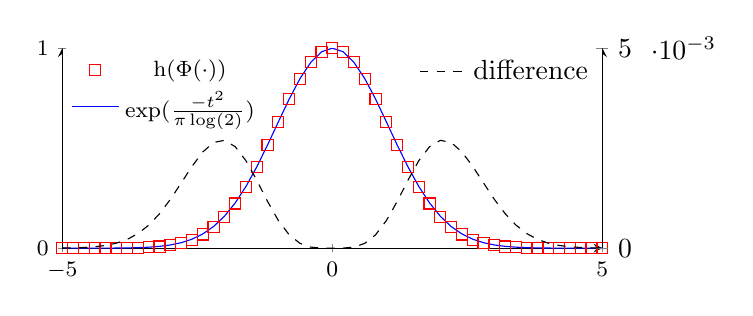
\begin{tikzpicture}

\begin{axis}[%
footnotesize,
scale only axis,
width=2.7in,
height=1.0in,
xmin=-5, xmax=5,
ymin=0, ymax=1,
xtick={-5,0,5},
ytick = {0,1},
axis y line = left,
axis x line = bottom,
legend style={ at={(0,1)}, anchor=north west, draw = none}]
]

\addplot [
color=red,
only marks,
mark=square,
mark options={solid}
]
coordinates{ (-5,6.64369e-06) (-4.8,1.72218e-05) (-4.6,4.2873e-05) (-4.4,0.000102503) (-4.2,0.000235365) (-4,0.000519064) (-3.8,0.0010995) (-3.6,0.00223711) (-3.4,0.00437257) (-3.2,0.00821083) (-3,0.0148147) (-2.8,0.0256873) (-2.6,0.0428103) (-2.4,0.0685917) (-2.2,0.105681) (-2,0.156615) (-1.8,0.223311) (-1.6,0.306444) (-1.4,0.40484) (-1.2,0.515021) (-1,0.631083) (-0.8,0.745014) (-0.6,0.847502) (-0.4,0.929133) (-0.2,0.981797) (0,1) (0.2,0.981797) (0.4,0.929133) (0.6,0.847502) (0.8,0.745014) (1,0.631083) (1.2,0.515021) (1.4,0.40484) (1.6,0.306444) (1.8,0.223311) (2,0.156615) (2.2,0.105681) (2.4,0.0685917) (2.6,0.0428103) (2.8,0.0256873) (3,0.0148147) (3.2,0.00821083) (3.4,0.00437257) (3.6,0.00223711) (3.8,0.0010995) (4,0.000519064) (4.2,0.000235365) (4.4,0.000102503) (4.6,4.2873e-05) (4.8,1.72218e-05) (5,6.64369e-06)
};
%\label{plots:approx_true}
\addlegendentry{$\mathrm{h}(\Phi(\cdot))$}

\addplot [
color=blue,
solid
]
coordinates{ (-5,1.03285e-05) (-4.8,2.54061e-05) (-4.6,6.02395e-05) (-4.4,0.00013768) (-4.2,0.000303323) (-4,0.000644146) (-3.8,0.00131859) (-3.6,0.00260182) (-3.4,0.0049487) (-3.2,0.00907298) (-3,0.0160344) (-2.8,0.0273151) (-2.6,0.0448534) (-2.4,0.0709961) (-2.2,0.108322) (-2,0.159311) (-1.8,0.22585) (-1.6,0.30863) (-1.4,0.406537) (-1.2,0.516189) (-1,0.631774) (-0.8,0.745348) (-0.6,0.847622) (-0.4,0.929159) (-0.2,0.981799) (0,1) (0.2,0.981799) (0.4,0.929159) (0.6,0.847622) (0.8,0.745348) (1,0.631774) (1.2,0.516189) (1.4,0.406537) (1.6,0.30863) (1.8,0.22585) (2,0.159311) (2.2,0.108322) (2.4,0.0709961) (2.6,0.0448534) (2.8,0.0273151) (3,0.0160344) (3.2,0.00907298) (3.4,0.0049487) (3.6,0.00260182) (3.8,0.00131859) (4,0.000644146) (4.2,0.000303323) (4.4,0.00013768) (4.6,6.02395e-05) (4.8,2.54061e-05) (5,1.03285e-05)
};
%\label{plots:approx_approx}
\addlegendentry{$\exp(\frac{-t^2}{\pi\log(2)})$}

\end{axis}

\begin{axis}[%
scale only axis,
width=2.7in,
height=1.0in,
xmin=-5, xmax=5,
ymin=0, ymax=0.005,
xtick={-5,0,5},
ytick = {0,0.005},
axis y line = right,
axis x line = none,
legend style={ at={(1,1)}, anchor=north east, draw = none}]
]

\addplot [
color=black,
dashed
]
coordinates{ (-5,3.68482e-06) (-4.8,8.18427e-06) (-4.6,1.73665e-05) (-4.4,3.51775e-05) (-4.2,6.79579e-05) (-4,0.000125081) (-3.8,0.000219088) (-3.6,0.000364708) (-3.4,0.000576126) (-3.2,0.000862153) (-3,0.00121977) (-2.8,0.00162773) (-2.6,0.00204316) (-2.4,0.00240434) (-2.2,0.0026417) (-2,0.00269602) (-1.8,0.00253851) (-1.6,0.00218519) (-1.4,0.00169772) (-1.2,0.00116807) (-1,0.000690885) (-0.8,0.000334143) (-0.6,0.000120243) (-0.4,2.60299e-05) (-0.2,1.71855e-06) (0,-0) (0.2,1.71855e-06) (0.4,2.60299e-05) (0.6,0.000120243) (0.8,0.000334143) (1,0.000690885) (1.2,0.00116807) (1.4,0.00169772) (1.6,0.00218519) (1.8,0.00253851) (2,0.00269602) (2.2,0.0026417) (2.4,0.00240434) (2.6,0.00204316) (2.8,0.00162773) (3,0.00121977) (3.2,0.000862153) (3.4,0.000576126) (3.6,0.000364708) (3.8,0.000219088) (4,0.000125081) (4.2,6.79579e-05) (4.4,3.51775e-05) (4.6,1.73665e-05) (4.8,8.18427e-06) (5,3.68482e-06)
};
%\label{plots:approx_error}
\addlegendentry{difference}

\end{axis}
\end{tikzpicture}

\caption{Analytic approximation ({\scriptsize $\stackrel{1}{\approx}$}) to the binary entropy of the error function by a squared exponential. The absolute error remains under $3 \cdot 10^{-3}$. \label{fig:trick}}
\end{figure} 

Most approximate inference methods for the problem of binary classification with
GPs produce a Gaussian approximation to the posterior distribution of $f$, the
latent function of interest. In the binary GP classifier, the entropy of $y$ given the corresponding value of $f$ 
can be expressed in terms of the binary entropy function, $\mathrm{h}[f]=- f\log f - (1-f)\log(1-f)$.
In particular,

\begin{align}
\ent[p(y\vert\x,\latfun)] &= \mathrm{h}\left[\Phi(\latfun(\x)\right]\,. \notag
\end{align}

Expectations over the posterior need to be computed. When using a Gaussian approximation to the posterior, for each $\x$, $\latfun_{\x} = \latfun(\x)$ will follow a Gaussian distribution with mean $\mu_{\x}$ and variance $\sigma_{\x}^2$. To compute \eqref{eqn:rearrangement} we have to compute two entropy quantities. The first term in \eqref{eqn:rearrangement}, $\ent[p(y\vert\x,\data)]$ can be handled analytically:
\begin{align}
        \ent[p(y\vert\x,\data)] &\stackrel{1}{\approx} \mathrm{h}\left( \int \Phi( \latfun_{\x} )  \mathcal{N}(\latfun_{\x}| \mu_{\x},\sigma_{\x}^2) d\latfun_{\x} \right) \notag \\ 
        &= \mathrm{h} \left( \Phi\left( \frac{\mu_{\x}}{\sqrt{\sigma^2_{\x} + 1}} \right)\right)\,, \label{ent_mean}
\end{align}

where $\stackrel{1}{\approx}$ denotes the Gaussian approximation to the posterior of $\latfun_{\x}$. The second term, \\ $\E_{\latfun \sim p(\latfun\vert\data)} \left[ \ent[p(\y\vert\x, \latfun)] \right]$ can be computed approximately as follows:

\begin{align}
        \E_{\latfun \sim p(f\vert\data)} \left[ \ent[p(\y\vert\x, \latfun)] \right] &\stackrel{1}{\approx}\int \mathrm{h}(\Phi(\latfun_{\x})) \mathcal{N}(\latfun_{\x}| \mu_{\x},\sigma_{\x}^2) d\latfun_{\x}\label{eqn:mean_entropy}\\
        &\stackrel{2}{\approx} \int \exp\left(-\frac{\latfun_{\x}^2}{\pi\ln2}\right) \mathcal{N}(\latfun_{\x}| \mu_{\x},\sigma_{\x}^2)d\latfun_{\x}\notag\\ 
        &= \frac{C}{\sqrt{\sigma_{\x}^2 + C^2}}\exp\left(-\frac{\mu_{\x}^2}{2\left(\sigma_{\x}^2 + C^2\right)}\right)\,,\notag
\end{align}

where $C=\sqrt{\frac{\pi\ln2}{2}}$. The integral in the left hand side of \eqref{eqn:mean_entropy} is intractable. By performing a Taylor expansion on $\ln \mathrm{h}(\Phi(\latfun_{\x}))$ (see the Supplementary material) we can see that it can be approximated up to $\mathcal{O}(\latfun_{\x}^4)$ by a squared exponential curve, $\exp(-\latfun_{\x}^2/\pi\ln2)$; this approximation is denoted {\scriptsize $\stackrel{2}{\approx}$}. Fig.\,\ref{fig:trick} depicts the striking accuracy of this simple approximation. The maximum possible error in the integral in \eqref{eqn:mean_entropy} that can be incurred is only 0.27\%. This happens when $\mathcal{N}(\latfun_{\x}| \mu_{\x},\sigma_{\x}^2)$ is centered at $\mu_{\x}=\pm 2.05$  with $\sigma_{\x}^2$ tending to zero. Now the convolution formula for Gaussians yields an closed form expression.

\begin{figure}[t]\centering
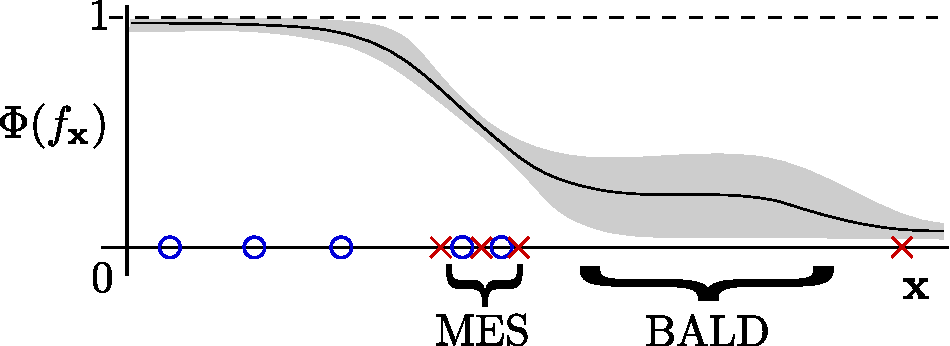
\includegraphics[scale = 0.5]{figs/BALD_eg.pdf} \\
\vskip-0.4cm
\caption{Toy classification example with a 1D input. Circles and crosses
are the data. We plot the mean and variance of the predictive
distribution. Maximum Entropy Sampling (MES, see Section \ref{sec:relatedWork})
samples from the region of highest marginal uncertainty, ignoring the
second term in \eqref{eqn:rearrangement}. BALD samples 
from the region of greatest model uncertainty i.e. the area with the largest 
shaded error-area. \label{fig:BALD}}
\end{figure}

To summarize, the BALD algorithm for Gaussian process active binary GP classification/ preference learning consists of two steps. First it applies any standard approximate inference algorithm (such as EP) to obtain the posterior predictive mean $\mu_{\x}$ and $\sigma_{\x}$ for each point of interest $\x$. Then, it selects the data $\x$ that maximizes the following objective function:

\begin{equation}
        \mathrm{h} \left( \Phi\left( \frac{\mu_{\x}}{\sqrt{\sigma^2_{\x} + 1}} \right)\right) - \frac{C}{\sqrt{\sigma_{\x}^2 + C^2}} \exp\left(-\frac{\mu_{\x}^2}{2\left(\sigma_{\x}^2 + C^2\right)}\right) \label{eqn:BALD}
\end{equation}

The BALD objective assigns high value to an $\x$ when the model is both uncertain in
the output ($\mu_{\x}=0$) and the there is high uncertainty in the parameters
($\sigma_{\x}^2$ is large). The second term prevents BALD from sampling in regions
where the model knows that the output is uncertain. Figure \ref{fig:BALD} illustrates
the differences between BALD and Maximum Entropy Sampling.
MES uses only the first term in \eqref{eqn:BALD}, and hence seeks data in an
uninformative region. BALD samples data from the region of greatest uncertainty in the model.

For most practically relevant kernels, the objective \eqref{eqn:BALD} is a smooth and differentiable function of $\x$, so should we be able to select items from a continuous feature space gradient-based optimization methods can be employed. We now describe how we perform inference in our multi-user model in order to get the distributions required for making predictions and active queries. 

